% "THE BEER-WARE LICENSE" (Revision 42):
%
% <danila.dolgopolov@mailbox.tu-dresden.de> wrote this file.   As long as you retain this notice you
% can do whatever you want with this stuff. If we meet some day, and you think
% this stuff is worth it, you can buy me a beer in return. Danila Dolgopolov

% The actualisation for the modern course Einführung in die Medieninformatik was done.
% Many thanks to the authors timklge@wh2.tu-dresden.de and @fsr for the opportunity to use their
% document as a template for this document!

\documentclass[12pt,landscape]{article}
\usepackage{multicol}
\usepackage{calc}
\usepackage{delarray}
\usepackage{amssymb}
\usepackage{amsmath}
\usepackage[landscape]{geometry}
\usepackage[utf8]{inputenc}
\usepackage{color}
\usepackage[compact]{titlesec}
\usepackage{graphicx}
\usepackage{listings}
\usepackage{color}
\usepackage{hyperref}
\usepackage{amsmath}
\usepackage{colonequals}
\usepackage[ddmmyyyy]{datetime}
\usepackage{fancyhdr}
\usepackage{setspace}

\definecolor{dkgreen}{rgb}{0,0.6,0}
\definecolor{gray}{rgb}{0.5,0.5,0.5}
\definecolor{mauve}{rgb}{0.58,0,0.82}
\def\code#1{\texttt{#1}} % define a func \code
\renewcommand{\THEYEAR}{\the\year}
\renewcommand{\dateseparator}{.}
\renewcommand{\headrulewidth}{0.4pt}
\hyphenation{Hin-ter-grund-ra-u-schen li-ne-a-re Grund-rei-zes Li-ni-en phy-si-ka-li-schen Zei-chen Farb-ra-um-um-rech-nung}

\lstset{ % set design for code sections
  language=Java,
  aboveskip=1mm,
  belowskip=1mm,
  showstringspaces=false,
  columns=flexible,
  basicstyle={\footnotesize\ttfamily},
  numbers=none, % (none, left, right)
  numberstyle=\tiny\color{gray},
  numbersep=3pt,
  keywordstyle=\color{blue},
  commentstyle=\color{dkgreen},
  stringstyle=\color{mauve},
  breaklines=true,
  breakatwhitespace=true,
  tabsize=4,
  frame=TB,
  rulecolor=\color{gray},
}
\pagestyle{empty}
\addtocontents{toc}{\protect\thispagestyle{empty}}
\geometry{top=1.3cm,left=1cm,right=1cm,bottom=0.7cm}

\pagestyle{fancy}
\fancyhead{}
\fancyfoot{}
\fancyhead[L]{\tiny FurTactics}
\fancyhead[C]{\tiny EMI \THEYEAR}
\fancyhead[R]{\tiny\thepage}

\setcounter{secnumdepth}{2}

\begin{document}
\footnotesize
\author{FurTactics\thanks {Danila Dolgopolov \href{mailto://danila.dolgopolov@mailbox.tu-dresden.de}{danila.dolgopolov@mailbox.tu-dresden.de}}}
\title{\Large Einführung in die Medieninformatik\\1. Semester}
\date{\normalsize \today}
\maketitle
\begin{multicols}{2}
    \renewcommand{\baselinestretch}{0.75}\normalsize
    \tableofcontents
\end{multicols}
\newpage
\begin{multicols}{3}

\section*{Allgemeines}
\addcontentsline{toc}{section}{Allgemeines}
\textbf{Informatik} ist die Wissenschaft, die sich mit den theoretischen Grundlagen, den Mitteln und Methoden der Informationsverarbeitung unter Einsatz von Computern beschäftigt
\subsection*{Aufgabenstellungen}
Berechenbarkeit (Lösen mathematischer Probleme), Unberechenbarkeit, Curchsche
These (Gleichwertigkeit aller Maschinenkonzepte), Chomsky-Hierarchie (Zusammenhang Automaten $\leftrightarrow$ Sprachgrammatik), Programmkomplexität, Programmverifikation
\subsection*{Medienkompetenz}
Medialitätsbewusstsein + Medienwissen, Medienspezifisches Rezeptionsmuster, Medienbezogene Genussfähigkeit (Bedürfnis nach Identifikation und Unterhaltung), Medienbezogene Kritikfähigkeit.\\
Medien: Mittel zur Speicherung von Information (Physisch oder Format, Text, Video, Audio)
\section{Audio}
\subsection{Diskretisierung}
\begin{itemize}
\item \textbf{Diskretisierung:} Festes Raster von Messpunkten gleichen Abstands wird festgelegt
\item Typischer Frequenzbereich 16 Hz - max. Hörfrequenz ca. 20kHz
\item \textbf{Analoge Audio-Signale:} Periodische Signale (Wellen), Amplitude (maximaler Wert): Lautstärke [dB], Frequenz: Tonhöhe, Phase bezeichnet den Zeitraum der Wiederholung, Obertöne sind Vielfaches einer Grundfrequenz
\item \textbf{Abtastrate:} die Dichte der Messwerte und wird als Samples pro Sekunde ausgedrückt
\item \textbf{Quantisierung:} Rundung der Messwerte auf das Raster / Darstellung  der Messwerte / Amplitude als Binärzahl
\item \textbf{Auflösung} ist die Anzahl Bits pro Sample. Sample: Ein Wert / eine Abtastung
\item \textbf{Abtastfehler:} Bei zu geringer Abtastrate kann sich ganz anderes Muster ergeben (konstanter Ton statt Schwingung)
\item \textbf{Nyquist-Shannon-Abtasttheorem:}\\$f_{abtast} > 2 \cdot f_{max}$, damit alle Signale ohne Informationsverlust dargestellt werden können
\end{itemize}
\subsection{PCM}
\begin{itemize}
\item \textbf{PCM} (Pulse Code Modulation): Analoge Spannung in digitale Daten verlustfrei aber fehlerbehaftet umwandeln (analoges Signal über analoge Filterstufe über zeitliche Abtastung über Quantisierung über Codierung zum binären Digitalsignal)
\item \textbf{Filter:} Tiefpass mit Grenzfrequenz $f_s$ -- höchste Signalfrequenz
\item Analogsignal wird mit dem linearen 3-Bit Wandler (8 Stufen) wertdiskretisiert, 2er-Komplementbildung
\item \textbf{Audio-CD:} 44100 Hz, 16 bit / Sample, 2 Kanäle (Stereo), d.h. Datenrate $=2\cdot\frac{44100}{s}\cdot\frac{16 Bit}{8\frac{Bit}{Byte}}=10\frac{MByte}{min}$. 12 cm Durchmesser, Umdrehungsgeschwindigkeit je nach Entfernung vom Mittelpunkt. Oberfläche besteht aus Pits und Lands (Löcher und Hügel). Hoch redundant, durch 16 bit pro Sample
\item \textbf{Blu-ray disc:} Kürzere Wellenlänge als bei DVD und CD, bessere Fokussierung, 36 MB/s, 25 GB pro Layer, MPEG-2 kodiert, beidseitige Laserabtastung
\item \textbf{RIFF} (Resource Interchange File Format): WAV (PCM) und AVI (AVID). Aufbau in Chunks (Chunk-ID, Chunk-Size, Chunk-Data)
\item \textbf{WAV:} 3 Chunks. \underline{Header-Chunk}: "RIFF" \textcolor{blue}{(4 Byte)}, Dateigröße \textcolor{blue}{4} (8 Bytes weniger als im System angezeigt), "WAVE" \textcolor{blue}{4}, \underline{Format-Chunk}: "fmt" \textcolor{blue}{4}, Größe des Formatblocks \textcolor{blue}{4} (16), Formatblock: Format \textcolor{blue}{2} (1 -- PCM), Kanäle \textcolor{blue}{2} (1 -- Mono, 2 -- Stereo), Samplefrequenz (Samples pro sec je Kanal) in Hz \textcolor{blue}{4} (bspw. 44100), Byte pro Sekunde \textcolor{blue}{4}, Byte pro Sample (Framegröße) \textcolor{blue}{2}, Bit pro Sample (Samplingtiefe) \textcolor{blue}{2}, \underline{Daten-Chunk}: "data" \textcolor{blue}{4}, Größe des Datenblocks \textcolor{blue}{4}, Datenblock
\item \textbf{PCM vs. Analog:} störresistene Übertragung möglich, verlustfreie Weiterbearbeitung, kostengünstige Schaltkreise verfügbar, aber Quantisierungsfehler (Rundung der Werte bei Einfügen in diskrete Tabelle) und Hintergrundrauschen bei der Aufzeichnung
\item \textbf{Quantisierungsfehler} maximal mit Betrag von $\frac{1}{2}$ der Quantisierungsstufe, hörbar als Rauschen
\item \textbf{Rauschen:} Einfluss der Codierung auf die Signalqualität, z.B. Quantisierungsfehler, ab 70dB unter Maximumpegel nicht hörbar
\item \textbf{DPCM} (Differential PCM): Differenz zwischen benachbarten Abtastwerten werden quantisiert und codiert, Geringere Wortbreite bei gleicher Qualität (max. Kompressionsfaktor 1 : 2)
\item \textbf{ADPCM} (Adaptive Differential PCM): periodisch neu berechnete Skalierung (leise: feine Einteilung, laut: grobe Einteilung), bessere Vorhersage durch Prädikator. Versucht, den weiteren Signalverlauf vorherzusagen, und kodiert und überträgt dann nur die Differenz zwischen tatsächlichem und vorhergesagtem Signal. Steile Signale teilw. nicht vollständig reproduzierbar. Bei CD-Qualität 4-fache Kompression, bis zu 32-facher Kompression bei starkem Qualitätsverlust
\item Weitere Formate: \textbf{MP3} (verlustbehaftete Kompression), \textbf{MOD} (Atari Musik), \textbf{AU}
\item \textbf{MIDI} (31250 Bit pro Sekunde), Byteweises Festlegen von Instrument, Tonhöhe, Dauer usw., Standardisiert, Erweiterbar
\end{itemize}
\subsection{Kompression}
\begin{itemize}
\item \textbf{Motivation:} Akustische Täuschung. Anforderungen:
\begin{itemize}
\item Geringe Toleranz erforderlich (Gehör genau, Abspielrate darf nicht länger als 10ms abweichen, Signal darf nicht wiederholt / augsetzt werden für 2ms, Gehörempfindlichkeit ist frequenzabhängig, Sprache: Inhalt wichtig [viel Semantik], bei Musik originalgetreue Wiedergabe wichtig)
\item Hörempflindlichkeit ist frequenzabhängig - Isophone: Stufen gleicher Lautstärke
\end{itemize}
\item \textbf{Wellenformcodierung} (ISDN, PCM, WAV): Einfache Technologie, \underline{Ziel}: Möglichst exakte Nachbildung
\item \textbf{Frequenzbereichcodierung} (MP3, WMA, OGG Vorbis): Komplexe psychoakustische Modelle, Frequenzbänder werden in unterschiedlicher Qualität übertragen, \underline{Ziel}: Möglichst genaue Nachbildung beim Weglassen von möglichst viel Information
\item \textbf{Parametrische Codierung} (GSM Sprachcodierung): Speicherung von Mustersequenzen (wie indexierte Bildformate), geeignet für Sprache (häufige (Teil)Widerholungen)
\item \textbf{Spracherkennung} (noch unausgereift) Erkennung $\rightarrow$ Textübertragung $\rightarrow$ Synthese, dann auch auf Musik übertragbar
\item \textbf{Redundanz:} Elemente ohne zusätzliche (neue) Information
\item \textbf{Irrelevanz:} Nicht wahrnehmbare Elemente
\item \textbf{Entropiecodierung:} Verlustfreie Kodierung, Eliminierung der Redundanz
\item \textbf{Reduktion:} Eliminierung von irrelevanten Daten
\item \textbf{Dekorrelation:} Umformung in andere Darstellung ohne Datenmenge zu ändern
\item \textbf{Codec} (Encoder / Decoder): Kombination verschiedener der oberen Techniken zu einem komplexen Modul
\item \textbf{Pipeline Encoder}: Signalaufbereitung (Abtasttheorem, Quantisierung), Signalzerlegung (Dekorrelation, Frequenzzerlegung o.ä.), Quantisierung (Perzeptionsmodelle, Reduktion), Entropiekodierung (Statische Modelle, z.B. ZIP)
\item \textbf{Mithörschwelle:} Laute Töne maskieren leise Töne, Frequenzanteile unterhalb der Kurve weglassen (laute Töne maskieren bis zu 20ms vor dem Ton und bis 200ms nach dem Ton, abhängig von Lautstärke, Frequenzverhältnis, zeitlicher Lage, Struktur/Dauer des Maskierens)
\item \textbf{Irrelevanzkodierung:} Herausfinden der Wahrnehmungsgrenzen, Anpassen der Quantisierung, Löschen der irrelevanten Teile. Dadurch mehr Quantisierungsrauschen, also Kompromiss aus Qualität und Bandbreite nötig
\item \textbf{Frequenzdarstellung:} Annäherung eines Rechtecksignals durch ungerade Vielfache einer Grundfrequenz
\item \textbf{Frequenzspektrum:} Graph mit Pegel [dB] auf Y-Achse und Frequenz auf X-Achse
\item \textbf{Interferenz:} Überlagerung von Wellen (Konstruktive: Addierend, Destruktive: Subtrahierend)
\item \textbf{Fourier-Transformation} (FFT) und \textbf{Diskrete Kosinus-Transformation} (DCT) erlauben die Umrechnung aus dem Signalraum (Frequenz über Zeit) in den Frequenzraum (Vorkommen von einzelnen Frequenzen)
\item \textbf{Subband Codierung:} Filterbank zerlegt Signal in Frequenzverbänder, Gesamtenergie des Signals meist ungleichmäßig verteilt, viele Bänder mit wenig Energie, wenig Bänder mit viel Energie, pro Frequenzband Maskierung bezüglich Irrelevanz (Hörschwelle, Verdeckung) und Quantisierung (Bitrate variabel), Bitstrommultiplexer erzeugt digitalen Datenstrom (inverse Filterbank setzt Signal fast perfekt zusammen)
\item \textbf{MP3:} Zerlegung in 32 Frequenzbänder, pro Teilband 18 Subbänder, Rauschen minimieren, Entropiekodierung, verdeckte Signalteile erkennen, optimale Codierung finden, 1152 Samples pro Frame, 30-230 kBit/s
% \item Audioverarbeitung: Veränderungen der Amplitude oder der Frequenz eines Filters, Lautstärke wird durch den Pegel bestimmt (0dB: 1 mW bei 0,775 Volt)
% \item Effektivwert $s_{effektiv} = \sqrt{\frac{1}{t}\int_{T}s^2(t)dt}$
% \item Gefahren der Pegelanpassung: Übersteuerung (die höchsten Signalwerte liegen außerhalb des quantisierten Bereichs, Clipping, dadurch Störsignale), Untersteuerung (Die höchsten Signalpegel liegen weit unter dem Maximalpegel, dadurch mehr Rauschen und geringerer Signal/Rausch-Abstand)
% \item Normalisierung: Anheben auf 0dB Pegel, Herstellung einer Symemetrie um den Nullpunkt
% \item Hüllkurve: Veränderung, um zeitlich beshränkte Pegelanpassungen vorzunehmen, Ein- und Ausblenden (Fading) durch Multiplikation mit einem Faktor zwischen 0 und 1
% \item Filter berechnen einen neuen Signalwert auf Basis eines Signalwerts und seiner Nachbarn (Analog: Kondensator, Spule, z. B. Hall, Digital: speziell in digitalen Signalprozessoren)
% \item Hochpass, Tiefpass: hohe/tiefe Frequenzen werden durchgelassen
% \item Bandpass: Nur ein Frequenzband wird durchgelassen, Bandsperre: Bestimmtes Frequenzband wird \textit{nicht} durchgelassen
% \item DSPs arbeiten im Frequenzraum
% \item Dynamik: Verhältnis zwischen dem größten und kleinsten Amplitudenwert in einem Zeitfenster, Dynamikkompression: Laute Stellen werden abgesenkt, leise Stellen angehoben
% \item Resampling: Abspielen des Signals mit einer anderen Samplefrequenz; doppelt so schnelles Signal dauert halb so lang und klingt eine Oktave höher
% \item Time stretching: Resampling mit periodischer Wiederholung, wodurch das Signal länger dauert, aber nicht in der Tonhöhe verändert wird
% \item Pitch shifting: Zeitgestrecktes Signal wird mit Originalfrequenz abgespielt
% \item Phasing, Chorus, Flanging: Verändern die Phase des Signals (Chorus: Addition phasenversetzter Kopien)
% \item Echo und Hall: Basieren auf Reflexion des Signals, bei Hall wird Raumaufbau mit einbezogen
\end{itemize}
\subsection{Klangsynthese}
\begin{itemize}
\item \textbf{Wave-Table ("Sampling") Verfahren:} Eine Periode wird für periodische Signale numerisch gespeichert und wiederholt abgespielt
\item \textbf{Additive Synthese:} Addieren von mehreren ($>$100) Sinus und Cosinus-Signalen (harmonischen Teiltönen) unterschiedlicher Frequenz kann beliebige Wellenformen erzeugen (Fourier-Synthese)
\item \textbf{Subtraktive Synthese:} Oszillator erzeugt ein obertonreiches Signal (z.B. Sägezahn), das durch Filter bearbeitet wird
\item \textbf{FM Synthese ("Keyboard"):} Modulieren einer hörbaren Trägerfrequenz durch eine hörbare Modulationsfrequenz erzeugt ebenfalls ein obertonreiches Signal, erlaubt günstige Synthesizer
\end{itemize}
\subsection{Hexadezimaldarstellung}
Z.B. die Abtastrate aus dem Datenblock in Hex-Editor ist \code{40 1F 00 00} $\rightarrow$ \code{00 00 1F 40} $=\\=1\cdot16^3+15\cdot16^2+4\cdot16^1+0\cdot16^0=8000$ Hz
\subsection{Gesamtgröße der Datei}
\textbf{Abtastfrequenz} [44100 Hz] $\cdot$ \textbf{Samplingtiefe} \newline[$16\frac{Bit}{Sample}=2\frac{Byte}{Sample}]\cdot$ Anzahl der \textbf{Kanäle} [2]\\
+ 44 Byte = Gesamtgröße in System \textbf{ODER}\\
+ 44 Byte - 8 Byte = Gesamtgröße in WAVE-Hex
\section{MCI}
MCI -- Mensch-Computer Interaktion
\begin{itemize}
\item \textbf{Menschliche Informationsverarbeitung:} visual overload, motorische Fertigkeiten
\item \textbf{Design für Diversität von Menschen:}  Erstellen von Produkten, Gebäuden und Umgebungen die von vornherein zugänglich sind für so viel wie mögliche Benutzer, d.h. auch für ältere Menschen, Menschen ohne und mit Behinderungen
\item \textbf{Sehschädigung:} Menschen mit Sehschädigung verwenden Sprachsynthese – Screenreader (Talkback für Android und VoiceOver für iOS), Spracheingabe und Gesten. Screenreader unterstützen auch Braillezeilen per Bluetooth
\item \textbf{Farbenblind:} Nicht nur Farbe, sondern auch geometrische Figuren zu verwenden, um wichtige Informationen zu vermitteln
\item \textbf{Hörbehinderung:} Untertitel und Spracherkennung, Sprachdolmetscher schreiben gesprochenes nach, Geräuscherkennung zur Visualisierung von akustischen Signalen
\item \textbf{Körperbehinderung:} Saug-Blaseschalter, Zwinkern, Eyetracking, Kopfgeste
\item \textbf{Ältere Menschen} (Sehbehinderung): Große Icons und Texte, hoher Kontrast, Spracheingabe und Sprachausgabe
\end{itemize}
\subsection{Interaktion}
WIMP (Benutzungsschnittstellen) -- Windows Icons Menus Pointers\\
\hypertarget{Gebrauchstauglichkeit}{\textbf{Gebrauchstauglichkeit}} ist das Ausmaß, in dem ein Produkt, System oder ein Dienst durch bestimmte Benutzer in einem bestimmten Anwendungskontext genutzt werden kann, um bestimmte Ziele \textbf{effektiv}, \textbf{effizient} und \textbf{zufriedenstellend} zu erreichen\\
\begin{enumerate}
\item \textbf{Eingabe/Quelle:} Tastatur, Mikrophon, Kamera und Speichermedium (SSD, HDD, CD, DVD)
\item \textbf{Verarbeitungseinheit:} Konverter (Filter, Kompression), Mischer, Splitter
\item \textbf{Ausgabe/Senke:} Lautsprecher, Monitor, Drucker und Speichermedium (SSD, HDD, CD, DVD)
\end{enumerate}
\subsection{Anforderungsanalyse}
Analyse der Aufgaben der Benutzer um kleinere Interaktionsschritte festzulegen
\subsubsection{Card Sorting}
Ermittelt wie Benutzer die Dinge benennen (Namen), gruppieren (Relationen) unf die Gruppen benennen (Kategorien)
\begin{itemize}
\item \textbf{Geschlossenes Card Sorting:} mit vorgegebenen Gruppen (für Erweiterungen)
\item \textbf{Offenes Card Sorting:} ohne vorgegebene Gruppe (für neues Design, aber führt zu sehr vielen Oberbegriffen)
\end{itemize}
\subsubsection{User-Centred Design (UCD)}
Kann man beliebig oft wiederholen:
Notwendigkeit $\rightarrow$ Kontext festlegen und verstehen (Card Sorting) $\rightarrow$ Beschreibung des Benutzers $\rightarrow$ Erstellen des Design (Prototypen/Mockup) $\rightarrow$ Design evaluieren (Heuristik) $\rightarrow$ System erfüllt Benutzeranforderungen\\
\textbf{Prototypen:} \underline{Low Fidelity:} Skizzen, Storyboard, Wireframe, Papier, \underline{Mitte:} Mock-Up, Wizard-of-Oz, \underline{High Fidelity:} Computereinsatz (Powerpoint), Implementierung der Interaktionstechniken\\
\textbf{Wizard-of-Oz:} eine Prototyping(Evaluations)-Technik, um technisch aufwändige Interaktionen vor deren Umsetzung zu evaluieren, bei der die Antworten des Systems durch eine Person (Wizard), statt durch die Software generiert werden
\section{Dart\&Flutter}
\subsection{Dart}
Dart ist die objekt-orientierte Sprache und unterstützt Hot Reload. Dart läuft an den Virtuellen Maschinen (VM) und ist unabhängig von der Architektur des Prozessors (Intel/AMD). Dart ist single threaded mit event loop und microtasks und dynamisch, d.h. der Speicherbedarf wächst und schrumpft automatisch\\
Einfaches Beispiel für den Aufruf der Funktion \code{print}:
\begin{lstlisting}
void main() {
  print('Hallo Welt'); /*print() ist eine Anweisung (Statement)*/}
\end{lstlisting}
\textbf{Deklaration der Variablen} ist eine Bekanntgabe des Namens und des Typs (Basistyps und Klasse), z.B. \code{int i; String s; bool ok;}. Alle Variablen außer \code{String}, \code{bool} und \code{int} können eine Referenz auf \code{null} sein\\
\textbf{Klasse} ist ein abstraktes Modell bzw. einen Bauplan für eine Reihe von ähnlichen Objekten\\
\textbf{Objekt} ist ein Exemplar eines bestimmten Datentyps oder einer bestimmten Klasse (auch "Objekttyp" genannt)\\
\begin{lstlisting}
class Square{
  double? length;
  double area(){return length!*length!;}}
void main(){
  Square quadrat = Square(); // Erstellung eines neuen Elements 
  quadrat.length=10;
  print("Area of rectangle is ${rectangle.area()}.");}
\end{lstlisting}
\subsubsection{Kontrollstruktur \code{switch}:}
\begin{lstlisting}
  ...
  switch (opnd) {
    case "-":
      result = "Subtrahieren";
      break;
    default: /*verpflichtet*/
      result = "Unbekannter Operator";
      break;
  }
\end{lstlisting}
\textbf{Funktionen mit optionalen Parametern:}\\
\code{void func(String 
s, [int n=0])}\\
\textbf{Funktionen mit benannten Parametern:}\\
\code{void func({required String s, required int n})} und der Aufruf: \code{func(s: "a", n: 1);}\\
\textbf{Listen:} \code{var list = [1, 2, 3];} und die Länge ist \code{list.length}\\
\textbf{Schleifen:} Mit \code{if}-Anweisung in \code{while}-Schleife kann man nach einer Bedienung \code{break;} to stop looping und \code{continue;} to skip to the next loop iteration\\
Mit \code{do\{;\} while()} kann man vor der Schleife etwas machen
\subsection{Apps}
Apps bestehen aus Widgets/Views, die Stateless oder Stateful sein können. Die wichtigsten Widgets sind Text, Textfield und Button
\begin{itemize}
\item \textbf{Ausgabetechnik:} Display, Lautsprecher, Vibrationsmotor
\item \textbf{Eingabetechnik:} Multitouch-Eingabe, Sensoren (Mikrofon, Kamera, Lagesensor, Gyroskop usw.), Funkschnittstellen (Wi-Fi, Bluetooth, NFC usw.)
\item \textbf{MEMS} (Micro-Electro-Mechanical-Systems) - Sensoren messen Bewegungen in eine Richtung oder eine Kreisbewegung für z.B. Lageänderung, Schrittzähler oder Indoor Navigation
\item \textbf{Annäherungsensor:} Display ausschalten bei Annäherung an Kopf während des Telefonierens
\item \textbf{Magnetsensor} (Kompass): Messung des Magnetfelds der Erde
\end{itemize}
\subsubsection{Digitale Barrierefreiheit}
4 Kriterien zur Softwareentwicklung:
\begin{enumerate}
\item \textbf{Wahrnehmbarkeit} (z.B. statt Pixeln Bildbeschreibung, Formeln; Untertitel)
\item \textbf{Bedienbarkeit} (z.B. Gesteneingabe führt zu Link, Tastaturunterstützung)
\item \textbf{Verständlichkeit} (z.B. Gebärdensprache, Leichte Sprache)
\item \textbf{Robustheit} (trotz Javascript, Einsatz von ARIA) 
\end{enumerate}
\subsubsection{Gesten}
\begin{itemize}
\item Streichen mit 1-3 Fingern kurz, doppelt oder mit Wartezeit
\item Schüttelgesten
\end{itemize}
\subsection{Flutter}
Flutter erweitert Dart um Widgets zur Entwicklung von interaktiven Benutzeroberflächen für Desktop, Browser und Mobiltelefone aus demselben Programm. Dafür nutzt er Klassen ("Blaupausen für Widgets" bestehen aus Datenstrukturen und 
Funktionen und beschreiben ein Objekt) und Objekte (konkrete Datenstrukturen und Funktionen)
\subsubsection{Klassen}
\code{MyApp()} ist ein Konstruktor, der ein Objekt der Klasse \code{MyApp} erstellt
\begin{lstlisting}
import "package:flutter/material.dart";

void main() => runApp(MaterialApp(
  home: Center(
    child: RichText(
      text: TextSpan(
        text: "Hello World",
),),),));
\end{lstlisting}
\textbf{Widgets:} Align, Column, Container, Icon, Image, Scaffold, Text usw.
\subsubsection{Buttons}
\begin{itemize}
\item \textbf{Radiobutton:} Benutzer wählen genau eine von mehreren Alternativen 
\item \textbf{ToggleButton:} Benutzer schalten den Zustand eines Schalters um
\item \textbf{Checkbutton:} Benutzer aktivieren oder deaktiveren eines oder mehrerer Schalter
\end{itemize}
\section{Evaluation}
Bewertung eines interaktiven Systems kann durch Experten oder Benutzer realisiert werden.  Ziel ist die Feststellung der Qualität der Benutzungsoberfläche nach der \hyperlink{Gebrauchstauglichkeit}{Gebrauchstauglichkeit}
\subsection{Heuristiken}
Verfahren, um Probleme zu lösen bei begrenztem Wissen und wenig Zeit\\
\textbf{Heuristik zur Barrierefreiheit:} Wahrnehmbarkeit, Bedienbarkeit, Verstehbarkeit und Robustheit
\subsubsection{Farbkontraste}
Wahrnehmung von Farbkontrasten wird beeinflusst durch Farbton, Helligkeit und Sättigung. Um den Kontrast zu definieren, verwendet man ein Farbmodell und vergleicht benachbarten Farbwerte\\
Standard RGB (Red, Green, Blue) (sRGB) definiert die Farben derart, dass eine der Farbkomponenten maximal sein 
kann und die anderen Null sind, um die entsprechende Farbwirkung zu erzielen. Also Farbwerte 0 … 255 (8 bit) bzw. $00_{16}$ … FF$_{16}$\\
\textbf{Der Farbkontrast} von zwei Farben laut der WCAG (Web Content Accessibility Guidelines) ist dann ausreichend, wenn ihr Helligkeitswert $L_1$ und $L_2$ das Verhältnis\hfill von\hfill $t=3$\hfill oder\hfill besser\hfill aufweist\hfill wobei\newline
\[t=\frac{L_1+0,05}{L_2+0,05}\]
\begin{itemize}
\item $t\geq4,5$ für normale und kleine Schrift (14 pt) für Level AA nach WCAG 2.0
\item $t\geq3$  für große oder fette Schrift (18pt bzw. 14 pt fett) für Level AA nach 
WCAG 2.0
\item $t\geq7$ für normale und kleine Schrift (14 pt) für Level AAA nach WCAG 2.0
\end{itemize}
Berechnung der \href{https://webaim.org/resources/contrastchecker/}{Luminanz} L im sRGB Farbraum:
\begin{equation*}
    L = 0.2126 \cdot \textbf{R} + 0.7152 \cdot \textbf{G} + 0.0722 \cdot \textbf{B} \newline
\end{equation*}
\begin{equation*}\small
     R_{sRGB} = \frac{R_{8bit}}{255} \textit{,   } G_{sRGB} = \frac{G_{8bit}}{255} \textit{,   } B_{sRGB} = \frac{B_{8bit}}{255}
\end{equation*}

\textbf{R} \colonequals
\begin{cases}
 \text{if } R_{sRGB} \leq 0.03928 & R = \frac{R_{sRGB}}{12.92} \\
 \text{else } & R=(\frac{R_{sRGB}+0.055}{1.055}) ^ {2.4}
\end{cases}

\textbf{G} \colonequals
\begin{cases}
 \text{if } G_{sRGB} \leq 0.03928 & G = \frac{G_{sRGB}}{12.92} \\
 \text{else } & G=(\frac{G_{sRGB}+0.055}{1.055}) ^ {2.4}
\end{cases}

\textbf{B} \colonequals
\begin{cases}
 \text{if } B_{sRGB} \leq 0.03928 & B = \frac{B_{sRGB}}{12.92} \\
 \text{else } & B=(\frac{B_{sRGB}+0.055}{1.055}) ^ {2.4}
\end{cases}
\subsection{Evaluationsmethoden}
Qualitäts- bzw. Gütekriterien für die Evaluation sind Objektivität (sind die Ergebnisse unabhängig vom Versuchsleiter?), Validität (gleiche Ergebnisse für denselben Gegenstand?), Reliabilität (mißt der Fragebogen was er messen soll?)
\begin{itemize}
    \item \textbf{Messgrößen:} Graphen, Zählungen (quantitative und thematische Analyse), Muster erkennen (qualitative Analyse)
    \item \textbf{Diagrammarten:} berichten über Daten und erfinden keine zusätzlichen Daten
    \item \textbf{Graphen aus mehreren Werten:} Gestapelte Balkendiagramme für bspw. Höchst-, Tiefst- und Mittelwerte
    \item \textbf{Deskriptive Statistik: Median:} \\
    max. 50\% Daten $<$ z, min. 50\% Daten $\leq$ z\\
    max. 50\% Daten $>$ z, min. 50\% Daten $\geq$ z
    \item \textbf{Fragebogen:} Vorgehensweise: Hypothese formulieren, Klärung der Variablen und Merkmale, Klärung, welche Messwerte erhoben werden können
\end{itemize}
\subsubsection{TLX}
TLX ist ein NASA Task Load Index zur Bestimmung des kognitiven Workloads. Der kognitive Workload ist die mentale Belastung, die mit einer Aufgabe verbunden ist\\
Der TLX Fragenkatalog ermittelt die subjektive mentale Belastung (Workload) bei der Bearbeitung einer Aufgabe oder im Umgang mit einem System. Teilnehmer beantworten 6 Fragen zur 
Effektivität:  \textit{Mental Demand} (MD): How mentally demanding was the task? \textit{Physical Demand} (PD): How physically demanding was the task? \textit{Temporal Demand} (TD): How hurried or rushed was the pace of the task? \textit{Performance} (OP): How successful were you in accomplishing what you were asked to do? \textit{Effort} (EF): How hard did you have to work to accomplish your level of performance? \textit{Frustration} (FR): How insecure, discouraged, irritated, stressed, and annoyed were you?
\section{Bild}
\subsection{SVG}
\begin{itemize}
\item EncapsulatedPostScript, Bildinformationen in speziellem Code, programmierbar, keine Alphakanäle, nur PostScript-Geräte
\item \textbf{SVG} (Scalable Vektor Graphics) in XML (Extensible Markup Language) für Bilder, Text, Animation, Formen (bspw. mit Inkscape malbar)
\item \textbf{Primitive:} \underline{circle-Element} mit Attributen cx, cy und r (CenterX und CenterY), \underline{ellipse} mit cx, cy, rx und ry, \underline{rect} mit x, y, width, height, \underline{line} mit x1, y1, x2, y2 ... , \underline{polygon / polyline} mit points = \code{"x1 y1 x2 y2 ..."}
\item \textbf{Pfade:} \lstinline|<path d=""></path>|, Möglich anzugeben: \textbf{M} x y (Move To), \textbf{L} x y (Linie zum Ziel malen), \textbf{H} x (Horizontale Linie), \textbf{V} y (Vertikale Linie), \textbf{Z} (Pfad schließen), \textbf{C} x1 y1 x2 y2 x y (wo x1 y1 x2 y2 -- Kontrollpunkte und x y -- Endpunkt) (Kubische Bézier-Kurve), \textbf{S} x2 y2 x y (wo x2 y2 -- Kontrollpunkt und x y -- Endpunkt) (Kubische Bézier-Kurve fortsetzen, vorherigen Kontrollpunkt spiegeln), \textbf{Q} x1 y1 x y (Quadratische Bézier-Kurve), \textbf{T} x y (Quadratische Bézier-Kurve fortsetzen, vorherigen Kontrollpunkt spiegeln), \textbf{A} rx ry x-axis-rotation large-arc-flag sweep-flag x y (wo rx ry -- Radien, large-arc-flag: der kurze (0) oder längere (1) Weg, sweep-flag: der obere (1) oder untere (0) Bogen und x y -- Endpunkt)  (Ellipsenbogen) - Groß geschriebene Buchstabe steht für absolute, kleine für relative Koordinaten\\Pfade beginnen immer mit moveto (M) und können mit Z enden
\end{itemize}
\begin{center}
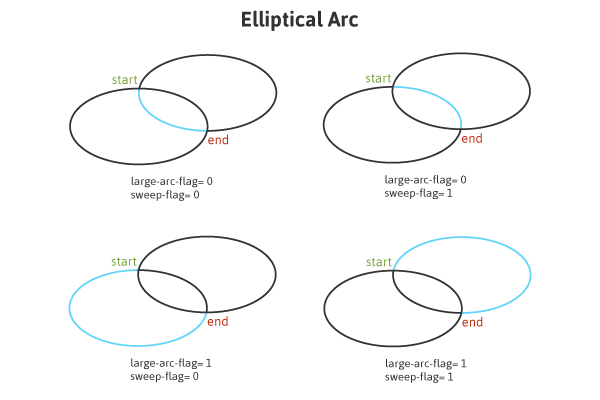
\includegraphics[height=100pt]{svg-path.png}\\
\tiny{\textit{(Bild: \href{https://www.sitepoint.com/closer-look-svg-path-data/}{Joni Trythall}, CC-BY)}}
\end{center}\\
\begin{itemize}
\item \textbf{Text:} text-Element mit x, y, font-size
\item \textbf{Image:} image-Element mit x, y, width, height, xlink:href
\item \textbf{Einfärben} von Formen mit \underline{fill}-Attribut und einer Farbe in Hex (z.B. \#FF0000) oder Name.
\item \textbf{Rand} malen mit \underline{stroke}-Attribut (enthält Farbcode) und \underline{stroke-width}-Attribut (Randbreite in Pixeln)
\item \textbf{transform}-Attribut gibt Rotation, Transformation, Skalierung oder Stauchung an: z. B. "translate(20, 150) scale(0.5) rotate(90,20,150) skewX(25) skewY(25)" - Bei Rotate dienen der zweite und dritte Parameter dabei als Rotationszentrum
\item \textbf{Clipping:} Beschränken eines zu zeichnenden Elements auf den Bereich, den ein anderes Element definiert
\item \textbf{Filter in SVG:} "Fotorealismus" durch Unschärfe, gezielte Einbringung von Bildstörungen o. ä.
\item \textbf{Blurring:} Unschärfefilter
\item Events in SVG mit JavaScript definiern (svg onload-Event, onclick-Event etc.)
\item \textbf{Animation} \begin{lstlisting}
<svg>
    <ellipse id="elli" cx="100" cy="100" rx="48" ry="90" style="fill:green;">
        <animate attributeType="XML" attributeName="rx" begin="0s" dur="6s" from="48"
            to="198" fill="freeze" />
    </ellipse>
</svg> 
\end{lstlisting}
\item In \lstinline|<defs>...</defs>| können SVG-Elemente definiert werden, die nicht gezeichnet werden, sondern mit \lstinline|<use xlink:href="#id">| später wieder benutzt werden
\end{itemize}
\subsection{Licht}
\begin{itemize}
\item Licht ist eine in Photonen gequantelte, 
transversale, elektromagnetische Welle
\item \textbf{Lichtgeschwindigkeit} im Vakuum $c = 299792458 \frac{km}{s}$ ist vom Medium, in dem sich das Licht bewegt, abhängig (meist Luft), $c = \lambda \cdot f$ ($\lambda$: Mediumskonstante, $f$: Frequenz des Lichts)
\item Frequenz ist Maß für \textbf{Energie} $E = hf = \frac{h c}{\lambda}$ (h ist das Planksche Wirkungsquantum mit ca. $h = 6.626 \cdot 10^{-34} J \cdot s$), d.h. je höher die Frequenz, desto energiereicher ist das Licht
\item \textbf{Frequenz} des sichtbaren Lichts beträgt ca. 400 nm - 780 nm, davor liegen die Frequenzbereiche von UV-Licht, Röntgen- und Gammastrahlung, darüber die von infrarotem Licht, UKW-Radio etc
\item Je höher die Frequenz, desto geringer die Wellenlänge (antiproportional)
% \item Lichtemission: Durch Gasentladung (z. B. Xenon Lampen), Photolumineszens (Phosphor "wandelt" einfallendes Licht in andere Wellenlänge um)
% \item Chemische Reaktion: Verbrennung (Flamme strahlt Licht)
% \item Phosphor: Elektronenbeschuss bringt Phosphor zum Leuchten
\item \textbf{Absorption:} Bspw. beim Durchlaufen einer farbigen Folie wird ein Teil des Lichtspektrums absorbiert
\item \textbf{Reflexion:} Ein Teil des Lichts wird beim Auftreffen auf eine Oberfläche reflektiert
\item \textbf{Additive Farbmischung:} Überlagerung von Licht mehrerer Emissionsquellen, Spektren werden addiert
\item \textbf{Subtraktive Farbmischung:} Einfallendes Licht fällt auf Filter (Absorption / Reflexion) ("Multiplikation mit Filterfunktion")
\item Gedruckte Farben erscheinen je nach Beleuchtung unterschiedlich (z.B. Gelb erscheint bei roter Beleuchtung rötlich)
\item \textbf{Farbtemperatur in Kelvin:} "Wärme" des Lichtes, je höher desto weißer -- Glühlampe ca. 2800K, Tageslicht: 6500K
\item Mensch "sieht" Lichtintensität, visuelle Wirkung, Konstrast, Formen, Bewegung
\item Sehen bzw. Licht beeinflusst Wachsamkeit, Wohlbefinden, innere Uhr usw.
% \item Spezielle Rezeptoren, spezieller Nervenpfad im Hirn
\item \textbf{Retina} im Auge mit Photorezeptoren besetzt, \textbf{Fovea} im Zentrum des Sehfeldes, \textbf{"Blinder Fleck"} des Auges ca. 1,75mm im Durchmesser (Gehirn "vervollständigt" das Bild)
\item Farbwahrnehmung in der Retina erfolgt durch Zapfen und Stäbchen (Zapfen: Farbwahrnehmung, Stäbchen: Schwarz/Weiß)
\end{itemize}
\subsection{Farbmodelle}
\begin{itemize}
\item Neben Helligkeit nimmt man als Hauptmerkmale Farbton und Sättigung wahr
\item Hirn teilt wahrgenommene Farben in weiß, grau, schwarz und verschiedene Farbtöne
\item \textbf{Farbwahrnehmung:} \underline{Helligkeit} (Luminance), \underline{Farbton} (Hue) und \underline{Sättigung} (Saturation) hauptsächlich
\item \textbf{RGB-Farbraum:} 256 Farbstufen pro Rot, Grün und Blau je 1 Byte, also $256^3 \approx$ 16,7 Millionen Farben (Truecolor)
\item CIE 1932: xyz-Kanäle, y: Wahrgenommene Helligkeit, x: rot/grün, z: blau/gelb-Unterschied
\item 128 Farbtöne (Hues), 130 Farbsättigungen (Saturation Levels), 16 (blau) - 26 (gelbe) Helligkeitswerte, also ca. 7 Millionen wahrnehmbare Farbnuancen
\item \textbf{Munsell Farbsystem} (Farbton hue, Helligkeit value, Sättigung chroma)
\item \textbf{HLS Farbsystem} (Hue, Luminance, Saturation)
\item \textbf{CMY Farbraum} (Cyan, Magenta, Yellow): $(r, g, b) = (1, 1, 1) - (c, m, y)$
\item \textbf{CMYK:} CMY mit Schwarz, damit Schwarz nicht aus Farbe gemischt werden muss (für Drucker toll)
\item \textbf{YUV:} Y: Helligkeit (s/w), U, V: Farbbalance
\item $YC_bC_r$: Y: Helligkeit, b: Blau, r: Rot
\item Farben in Text: Hervorhebung, sparsam (auffällige) Farben einsetzen
% \item Räumliches Sehen durch Augenabstand (Fusion, Disparität) zum Erkennen von relativer Größe, Perspektive, Beleuchtung
% \item Hirn bildet 3D-Modell (Fusion): Unterdrückung unvereinbarer Regionen, bei Überlagerung wechselt unvereinbares linkes / rechts Bild
% \item Räumliches Sehen: Fokus (Raumpunkt, auf den die Augen fokussiert sind), Retinale Position (relative Position zur optischen Achse), Mentales Auge: Fusion kombiniert Information
% \item Disparität: Unterschied von fusionierten Punkten kann zur Berechnung der relativen Position benutzt werden
\end{itemize}
\subsection{Digitale Bilder}
Digitale Bilder bestehen aus Pixeln ($w \frac{\text{Pixel}}{\text{Zeile}} \cdot h \text{ Zeilen}$), die pro Pixel meist 1-32 Bit Farbinfos beinhalten (Farbtiefe des Bildes) (ab 24 bit: \textbf{TrueColor})
\begin{itemize}
\item \textbf{Indizierte Farbformate:} Zu Beginn des Bildes Farbtabelle, danach wird jede Farbe mit einem Index auf die Farbtabelle angegeben (sinnvoll bei wenigen verwendeten Farben)
\item \textbf{Chroma Subsampling} bei YUV und $YC_bC_r$ (4 : 2 : 2): Halbe Auflösung für g/b (U) und magenta/yellow (V)-Kanäle
\item \textbf{Alphakanal:} Transparenzangabe
\item dpi/ppi: dots per inch/pixels per inch (Pixel pro Zoll, $1 \textit{ inch} \approx 2,54\textit{ cm}$)
\item Monitor ca. 72 dpi, Laserdrucker ca. 1200 dpi
\end{itemize}
\subsection{Digitale Bildformate}
\begin{itemize}
\item \textbf{Histogramm:} Gibt Verteilung der Graustufen von 0 bis 1 des Schwarzwertes an
\item \textbf{Bildfilter:} Beispielsweise Weichzeichner (lineare Mittelwertbildung aus Nachbarn um einen Pixel herum)
\item \textbf{GIF} (Graphics Interchange Format): Animierbares farbindiziertes Bildformat mit 256 Farbstufen (Farbtiefe bis zu 8 Bit), kein Alphakanal, verlustbehaftete Kompression
\item \textbf{PNG} (Portable Network Graphics): verlustfreie Kompression im Gegensatz zum GIF, Alphakanäle, freies Format, keine Animation, Farbtiefe bis zu 48 Bit, nicht für Fotos geeignet (verlustfreie Kompression zu schwach), Interlacing (Zunächst werden nur einige Zeilen des Bildes übertragen und dadurch eine Vorschau möglich, bevor das ganze Bild übertragen ist)
\item \textbf{JPEG} (Joint Photographic Experts Group): Verlustbehaftete Kompression u.a. mit Huffmann-Kodierung, Bildung von 8x8-Blöcken -- führt zu Blockbildung, JPEG-2000 als Nachfolger mit geringerer Artefaktbildung -- Farbraumumrechnung in YUV, Tiefpassfilterung \& Unterabtastung der Farbdifferenzsignale U, V (verlustbehaftet 4 : 2 : 2, s.o.), Quantisierung, Umsortierung, Huffmann-Kodierung. Gut geeignet für Fotos, nicht gut für alles andere (Diagramme etc)
\item \textbf{JPEG2000:} basiert auf XML, ermöglicht Rechtemanagment, verschieden starke Komprimierung in verschiedenen Bildteilen, Interlacing-Support
\item \textbf{TIF} (Tagged Image Format): mehrere Farbräume wie RGB, LAB, verlustfreie Komprimierung mit LZW-Algorithmus (Lempel, Ziv, Welch), können von den vielen Browsern nicht  dargestellt/verarbeitet werden
\item \textbf{PSD} (Adobe Photoshop): Kanäle, Bearbeitungsschritte, Text wird nicht gerastert, kann von vielen Programmen nicht gelesen werden
\end{itemize}
\subsection{Vektorgrafik}
\begin{itemize}
\item Beschreibung des Bildes mittels Formen wie Kreisen (Radius), Rechtecken (Höhe und Breite), Liniensegmenten (Endpunkte) usw. und nicht durch Pixel (Bsp.: SVG)
\item \textbf{Transformationen} (Rotation, Translation, Skalierung, Scherung) können mittels der Multiplikation des alten Vektors mit einer Matrix und der Addition eines neuen Vektors ausgedrückt werden
$\begin{pmatrix}
x' \\ y'
\end{pmatrix} = \begin{pmatrix}
a & b \\ c & d 
\end{pmatrix}\begin{pmatrix}
x \\ y
\end{pmatrix} + \begin{pmatrix}
e \\ f
\end{pmatrix}$
\item[] Translation: $\begin{pmatrix}
x' \\ y'
\end{pmatrix} = \begin{pmatrix}
1 & 0 \\ 0 & 1 
\end{pmatrix}\begin{pmatrix}
x \\ y
\end{pmatrix} + \begin{pmatrix}
\Delta x \\ \Delta y
\end{pmatrix}$
\item[] Rotation: $\begin{pmatrix}
x' \\ y'
\end{pmatrix} = \begin{pmatrix}
\cos \alpha & -\sin \alpha \\ \sin \alpha & \cos \alpha 
\end{pmatrix}\begin{pmatrix}
x \\ y
\end{pmatrix} + \begin{pmatrix}
0 \\ 0
\end{pmatrix}$
\item[] Scherung: $\begin{pmatrix}
x' \\ y'
\end{pmatrix} = \begin{pmatrix}
1 & s \\ 0 & 1
\end{pmatrix}\begin{pmatrix}
x \\ y
\end{pmatrix} + \begin{pmatrix}
0 \\ 0
\end{pmatrix}$
\item[] Skalierung: $\begin{pmatrix} x' \\ y' \end{pmatrix} = \begin{pmatrix}
a & 0 \\ 0 & b
\end{pmatrix}
\begin{pmatrix} x \\ y \end{pmatrix} + \begin{pmatrix}
0 \\ 0
\end{pmatrix}$
\item \textbf{Bezierkurven} dritten Grades / kubische Kurven: Kurven nach dem Format:
$\begin{pmatrix} x(t) \\ y(t) \end{pmatrix} = (1-t)^3 \begin{pmatrix} x_0 \\ y_0 \end{pmatrix} + 3t(1 - t)^2 \begin{pmatrix} x_1 \\ y_1 \end{pmatrix} + 3t^2(1 - t) \begin{pmatrix} x_2 \\ y_2 \end{pmatrix} + t^3
\begin{pmatrix} x_3 \\ y_3 \end{pmatrix}$ mit $t\in[0,1]$.
Dabei sind $\begin{pmatrix} x_0 \\ y_0 \end{pmatrix}$ und $\begin{pmatrix} x_3 \\ y_3 \end{pmatrix}$ die Start- bzw. Endpunkte der Kurve und $\begin{pmatrix} x_1 \\ y_1 \end{pmatrix}$ sowie $\begin{pmatrix} x_2 \\ y_2 \end{pmatrix}$ definieren die Tangenten an diesen Punkten.
\item \textbf{de Casteljau-Schema:} $t = \frac{1}{4}$
\item \textbf{Gruppierung} von einzelnen Formen, damit Transformation auf alle Elemente in der Gruppe angewendet werden können
\item \textbf{Tiefe:} Definierung einer Tiefenkoordinate, damit die Überlagerungsreihenfolge bei verdeckenden Formen definiert werden kann
\item TrueType-Fonts: Die Kontur von Zeichen werden durch Bezierkurven beschrieben, wird dann gefüllt
\item Meta Font (\LaTeX): Glyphenkontur wird durch interpolierende Kurve beschrieben
% \item Rasterisierung: Übersetzung von Vektorgrafik in Pixelgrafik (durch Test jedes Bildpunkts, ob er in einer Form liegt oder durch zeilenweises Abtasten [Sweepline], oder durch Abtasten jeder Form und Setzen der ausgefüllten Pixel)
% \item Dropouts (bei TrueType-Fonts): Nur halb ausgefüllte Pixel werden falsch als nicht gegeben gesetzt, daher setzen TrueType-Abtaster einen Pixel zwischen zwei anderen Pixeln auch dann, wenn zwischen diesen Pixeln zwei Konturlinien der Glyphe liegen (aber nur dann, wenn beide Konturen in beide Richtungen fortgesetzt werden)
\end{itemize}
\section{Wahrnehmung}
\begin{itemize}
\item "Wahrnehmung ist der Prozess, durch den Lebewesen Kenntnisse über ihre Umgebung und über sich selbst in Beziehung zur Umgebung gewinnen. Sie ist der Anfang allen Wissens."
\item \textbf{Motivation:} Notwendige Daten an menschliche Warnehmung anpassen, um Platz zu sparen (z.B. nicht wahrnehmbare Töne bei Audio). Ergonomisch physische Dinge gestalten, Gestaltung von Benutzerschnittstellen, Layout etc. auf Menschen optimieren
% \item $Reiz \rightarrow Sensor (analog) \rightarrow Filter \rightarrow Quantisierung (Digitalisierung) \rightarrow Filter (digital) \rightarrow Kompression \rightarrow Codierung \rightarrow Speichermedium$
% \item $Speichermedium \rightarrow Decodierung \rightarrow Dekompression \rightarrow Filter (digital) \rightarrow Rekonstruktion \rightarrow Filter (analog) \rightarrow Display (analog) \rightarrow Reiz (beim Mensch)$
% \item Wie funktioniert Reiz? Wie werden Reize beim Menschen wahrgenommen (Visuell, Akustisch, Haptisch, Gustorisch / Geschmack, Olfaktorisch / Geruch), Multimedial: Sprache und Deixis, Multimodal: Gedächtnisleistungen. Wie stark wird welcher Reiz wahrgenommen? Wie gleicht man produzierten Reiz mit echtem Reiz ab?
\item $\leftrightarrow$ Reize $\leftrightarrow$ (Psychophysik) $\leftrightarrow$ Wahrnehmung $\leftrightarrow$ (Psycho-, Neuro- und Biophysiologie) $\leftrightarrow$ Neuronale Prozesse (Physiologie) $\leftrightarrow$
\item \textbf{Funktionale Physiologie:} Erkenntnisse durch Patienten mit verletzten Gehirnen, elektrische Störungen von außen, durch teilweise Einschläferung, mit Elektro-Enzephalographie, Magneto-Enzephalographie
\end{itemize}
\subsubsection{Psychophysikalische Skalierung}
\begin{itemize}
\item \textbf{Wahrnehmung ist relativ:} Größe / Helligkeit 
\item \textbf{Auflösung des Auges:} $\delta$ minimaler Sehwinkel, bei dem 2 Linien im Abstand $s$ getrennt erkannt werden\[s = 2a \cdot \tan{\frac{\delta}{2}}\] mit Betrachtungsabstand $a$
\item Wahrnehmung der Länge erfolgt logarithmisch (bei längeren Strukturen müssen Unterschiede größer sein)
\item Wahrgenommene Skalen für Größe von Kreisen ist abhängig vom Radius
% \item Spitze Winkel werden unter- und stumpfe Winkel überspitzt
\item \textbf{Reizschwelle $R_0$:} kleinster wahrnehmbarer Reiz (z.B. Helligkeit des dunkelsten, noch erkennbaren Sterns am Nachthimmel), quantitatives Maß (z.B. Pa beim Hören) 
\item \textbf{Unterscheidungsschwelle $\Delta R$:} kleinster Unterschied von einem Grundreiz (z.B. Helligkeitsdifferenz für einen Punkt, den man gerade noch auf einem grauen Hintergrund wahrnehmen kann), qualitatives Maß 
\item \textbf{Messverfahren} erfordern Wahrnehmung von Reizen: Methode konstanter Reize (Zufällige Wiedergabe von verschieden starken Reizen, der zu 50\% erkannte Reiz ist die Reizschwelle -- sehr genau, langsam), Herstellungsmethode (VP stellt den Reiz selbst ein -- ungenau, schnell), Grenzmethode (Reiz erhöhen bis ihn VP erkennt -- genau, langsam)
\item Empfindungsstärke $\Psi$, Intensität des Grundreizes $R_0$, Unterscheidungsschwelle $\Delta R$, $k$ von Sinnesmodalität\hfill abhängige\hfill Konstante\hfill und\newline $c$ -- Proportionalitätskonstante für die Skalierung
\item \textbf{Webersche und Weber-Fechnersche Gesetze:}\\
\[\frac{\Delta R}{R} = k \text{ und }\Psi(R) = c \cdot \ln{\frac{R}{R_0}}\]

\item Quadriert man die Stärke des Grundreizes, dann verdoppelt sich die Empfindungsstärke
\item \textbf{Stevensches Potenzgesetz:} \[\Psi(R) = c \cdot (R - R_0)^n\]Entscheidend ist der Parameter $n$. Für Helligkeit gilt $n = 0.3$, für ein Gewicht $n = 1.5$, für die Länge einer Linie $n = 1.0$
\item Empfindungsstärken wie Lautstärke: Verwendung einer logarithmischen Einheit wie Dezibel (Konstante $k$ wird weggelassen)
\item Eine Erhöhung um 10dB bewirkt eine Verdopplung der Lautheit
\item \textbf{Bel:} Logarithmus des Quotienten zweier Leistungen \[Pegel = \lg \frac{R}{R_0} \text{ [Bel]}\]
\item \textbf{Dezibel:} Zehntel eines Bels  \[Pegel=10 \cdot \lg \frac{R}{R_0} =10 \cdot \lg\left(\frac{A^2}{A_0^2}\right)=20 \cdot \lg\left(\frac{A}{A_0}\right)\] [dB] und $A_0=2\cdot10^{-5}$ Pa heißt der Luftschall
\end{itemize}
\subsubsection{Gestalt}
\begin{itemize}
\item \textbf{Wahrnehmung:} Extraktion elementarer Merkmale (Kanten, Farbe) $\rightarrow$ Präattentive Verarbeitung (Erkennen elementarer Bestandteile) $\rightarrow$ Attentive Verarbeitung (Konstruktion des Gesamten)
\item Wörter eines Textes werden nicht Buchstabe für Buchstabe wahrgenommen (Auge liest 6-8 Buchstaben und springt dann weiter (ca. 20 ms)), Hören funktioniert ähnlich (Speicherdauer ca. 1,5 s)
\item \textbf{Gesetz der guten Gestalt/Prägnanz:} Übergeordnetes Gesetz zur Wahrnehmung von Gegenständen, Zusammenführung von prägnanten Einzeleindrücken zu Gestalt
\item \textbf{Gesetz von Figur und Grund:} Figur wird als vor dem Hintegrund stehend wahrgenommen, Figur und Grund kann nicht gleichzeitig wahrgenommen werden
\item \textbf{Gesetz der Gleichheit:} Ähnliche Dinge erscheinen zu zusammengehörigen Gruppen geordnet
\item \textbf{Gesetz der Nähe:} Dinge, die sich nebeneinander befinden, erscheinen als zusammengehörig
\item \textbf{Gesetz der Geschlossenheit:} Von Linien umschlossene Gegenstände werden als zusammengehörig empfunden
\item \textbf{Gesetz des weiterführenden oder gleichen Verlaufs:} Bruchstücke reichen zum Bilden von Gestalten aus
\item \textbf{Gesetz der Symmetrie:} Symmetrische Gebilde werden als Figur wahrgenommen
\item \textbf{Gesetz des gleichen Schicksals:} Objekte, die sich mit gleicher Geschwindigkeit bewegen, werden als zusammengehörig empfunden
\item \textbf{Gesetz der Erfahrung:} Wiedererkennen von bestimmten Formen
\item Gestaltgesetze betreffen die präattentive Wahrnehmungsphase und finden vor allem z.B. bei der Interfacegestaltung Anwendung (Gestaltung von Icons, Bedienoberflächen)
\item Bei rivalisierenden präattentiven Prozessen kommt es zu Wahrnehmungstäuschungen, Linien werden gebogen oder dynamische Effekte werden erzeugt
% \item Geone: Dreidimensionale Grundformen werden präattentiv anhand der Kantenanordnung erkannt und dann attentiv zu einem Gegenstand wie einem Tisch zusammeninterpretert
\end{itemize}
\section{Kodierung}
\subsection{Signale}
Ein \textbf{analoges Signal} ist die Änderung einer physikalischen Größe entsprechend einem Messwert der zu übertragenen Information\\
Ein \textbf{digitales Signal} orientiert sich an einem festen Raster und gibt Werte aus einem "endlichen Vorrat" möglicher Werte an (diskreter Wert)\\
Analoge Signale sind störanfällig gegenüber Rauschen (Schallplatte, Rundfunk, Foto). Digitale Signale sind unempfindlich gegenüber gegen Störsignale, solange das Signal nicht vollständig verfälscht wird oder ausfällt\\
\textbf{Bitgruppen:} 1 bit: Bit, 3 bit: Triade (Oktalsystem), 8 bit: Byte, 16 bit: Word, 32 bit: Doubleword, 64 bit: Quadword
\subsection{Entropie}
\textbf{Entropie} $H$ ist ein Maß für den durchschnittlichen Informationsgehalt einer Nachrichtenquelle. Es gilt:
\[ H = - \sum_{i}p_i \cdot \log_2(p_i) \]
Wobei $p_i$ Auftrittswahrscheinlichkeit des Zeichens $g_i \in A$ ist und $A$ das Alphabet. Maßeinheit ist 1 Bit.
\subsection{Umrechnung}
\underline{Dezimal zu Hexadezimal}: Zahl durch 16 teilen, Rest als Ziffer nehmen. Dann das Ergebnis der Zahl durch 16 für den nächsten Schritt verwenden (also erneut durch 16 teilen). Zahl am Ende rückwärts nehmen\\
\underline{Hexadezimal zu Dezimal}: Zahl von rechts nach links nehmen, erste Ziffer mit $16^0$ multiplizieren, zweite Ziffer mit $16^1$ usw.\\
$2^{10}$ -- Kibibyte, $2^{20}$ -- Mebibyte, $2^{30}$ -- Gibibyte usw. 
\subsection{Huffmann und Fano}
\begin{itemize}
\item \textbf{Alphabet:} Definiert lineare Ordnung auf Zeichen. Ein Binärcode ordnet jedem Element eines Alphabets ein Element eines Binäralphabets zu
\item \textbf{Fano-Bedingung/Präfixfreiheit:} Kein Zeichen ist Beginn eines anderes Zeichens
\item \textbf{Mittlere Länge} eines Binärzeichens $i$ mit der Länge $N_i$ wird berechnet als: \[L = \sum_{i} p_i \cdot N_i\] 
\item \textbf{Shannon's Theorem:} Es gilt immer $H \leq L$, Differenz kann sehr klein sein, die Differenz \[R = L - H\] wird \textbf{Redundanz} bzw. Nachrichtenanteil, der nicht unmittelbar zur Information beiträgt genannt
\item \textbf{Fano-Kodierung:} Zunächst werden die Zeichen so auf 0 und 1 verteilt, dass die Summe der jeweiligen Wahrscheinlichkeiten möglichst gleich groß ist. Dies wird dann so lange wiederholt, bis jedes Zeichen einen eigenen Code hat
\item \textbf{Huffmann-Kodierung:} Es wird ein binärer Baum angelegt, dessen Blätter zunächst das Alphabet sind. Die beiden Zeichen mit der geringsten Wahrscheinlichkeit werden genommen und mit 0 und 1 beschriftet
\end{itemize}
\section{Text}
\subsection{Zeichensätze}
Zeichensatz definiert Zuordnung von Zahlen zu Zeichen
\begin{enumerate}
\item \textbf{ASCII:} 7-bit-Zeichensatz (128 Zuordnungen), 0-31 Steuerzeichen. Neuere Zeichensätze sind meist abwärtskompatibel (Erste 128 Zuordnungen entsprechen ASCII)
\item \hypertarget{latin}{\textbf{ISO-8859-1...16:}} 8-bit-Zeichensätze (256 Zuordnungen), 0-127 ist ASCII, Sonderzeichen wie deutsche Umlauts in allen Latin-Varianten an selber Stelle (-1: Latin1 westeuropäisch, -2: Latin2 osteuropäisch, -5: Kyrillisch, -6: Arabisch, -7: Griechisch, [...], -15: Westeuropäisch mit Eurozeichen)
\item \textbf{Unicode:} Internationaler Zeichensatz. Verschiedene Standards: UCS-2 mit 2 hoch 16 Bit Zeichen, UCS-4 mit doppelt so vielen Ebenen. Unicode 5 kennt 99 089 Zeichen. Formate:
\begin{itemize}
\item \textbf{BigEndian:} Höchstes Byte steht ganz rechts (TCP/IP, JPEG, PNG),\\
\textbf{LittleEndian:} Höchstes Byte steht ganz links (Intel/x86, USB, PCI)
\item \textbf{UTF-32:} Immer 4 Bytes für ein Zeichen
\item \textbf{UTF-16:} 2 Bytes pro Zeichen mit Möglichkeit für mehr, wenn in ersten 2 Bytes spezille Surrogate-Kodierung benutzt wird
\item \textbf{UTF-8:} Wichtigstes Unicode-Format, weit verbreitet z.B. für XML. Besteht aus einem Byte pro Zeichen, das ASCII ist, wenn aber das oberste Bit gesetzt ist, dann ab 128 mit 2 Bytes, ab 2048 -- 3 Bytes und ab 65536 -- 4 Bytes\\ \underline{Aufbauschema}: Höchstes Bit ist nicht gesetzt, wenn es nur ein ASCII-Zeichen ist und somit nur aus einem Byte besteht. Ist das höchste Bit gesetzt, gibt die Anzahl der dann folgenden Bits die 1 sind an, aus wie vielen Bytes das Zeichen besteht. Ist das erste Byte z.B. 11100000, folgen noch zwei weitere Bytes für das gleiche Zeichen. 
\end{itemize}
\end{enumerate}
\subsection{Schrift}
\subsubsection{Eigenschaften}
\begin{center}
\includegraphics[height=100pt]{typografie.png}\\
\tiny{\textit{(Bild: Brian Ammon, CC-BY)}}
\end{center}
\begin{itemize}
\item Höhe wird in Punkt angegeben. Ein Punkt ist meist 1/72 Zoll (TeX, DTP/PostScript), 1 Pica sind 12 Punkte.
\item \textbf{Schriftstärke} (mager, normal, fett), \textbf{Schriftbreite} (schmal, normal, breit), \textbf{Schriftlage} (normal, kursiv)
\item \textbf{Vektorschriften:} Definition durch Vektoren,\\
\textbf{Rasterschriften:} Definition durch Pixelgrafik für je ein Zeichen
\item \textbf{Serifen:} Helfen bei Lesbarkeit, sollte nur bei Fließtext benutzt werden
\item \textbf{Kerning:} Anpassung von Zeichenabständen bei parallelen Diagonalen ("BRAVO": Zusammenrücken von A und V), Definition pro Buchstabenpaar. Kann doof sein bei geringen Abständen
\end{itemize}
\subsubsection{Braille-Schrift}
Von Louis Braille 1820 für Blinde entwickelt, für viele natürliche Sprachen verfügbar. Gibt Zeichen als fühlbare Punkte auf dem Papier wieder (6 - 8 Punkte kodieren ein Zeichen). Spezielle Schreibweisen für Formeln, Musik o.ä.
\subsubsection{Absätze}
Absatzformat gibt Abstände und Einrückungen an. Möglich sind z.B. Blocksatz (Automatische Anpassung des Wortabstandes, sodass stets ganze Zeile gefüllt wird), Flattersatz/Mittelachsensatz (optimale Wortabstände). Seitenlayout: Kopf, Rumpf, Fuß
\subsubsection{Auszeichnungssprache (ML)}
Markup Language ist eine maschinenlesbare Sprache für die Gliederung und Formatierung von Texten. Bsp.: \LaTeX, HTML
\subsubsection{Formate}
Eigenschaften: Editierbar? WYSIWYG (What You See Is What You Get)? Lesbar? Medien einbindbar? Funktionsumfang? Programmierbar? Barrierefreiheit?
\begin{itemize}
\item \textbf{Plain}
\item \textbf{Rich Text .rtf} (Microsoft), eigene Definition für Medien, nicht programmierbar, alt, MS Word ist WYSIWYG-Editor\begin{lstlisting}
{\rtf Hallo \par {\i Dies} war kursiv.
\par Noch ne Zeile.}\end{lstlisting}
\item \textbf{\LaTeX\ .tex} (frei), voll programmierbar, nicht WYSIWYG (wirft PDF o.ä. aus), Medien einbindbar, gute Formelsetzungsbibliotheken, vielseitig und toll, aber kompliziert
\item \textbf{PDF} (Adobe), baut auf Postscript auf, Layout-Treu, Rechtemanagment, Einbetten von Schriften problematisch, kaum editierbar, wird aus anderen Formaten generiert. PDF/A ist archivierbar, PDF/UA ist barrierefrei
\item \textbf{HTML:} Trennung von Struktur und Style mit CSS, Scripting (Document Object Model: Abbildung des XML-Baums auf JavaScript), programmierbar, kein WYSIWYG, Plugins
\end{itemize}
\section{XML}
\begin{itemize}
\item Medien in Dokumenten definieren sich durch \textbf{Inhalt} (Semantik), \textbf{Struktur} (Syntax) und \textbf{Präsentation} (lexikalische Information)
\item Für Arbeiten mit HTML bedient man sich der Sprache, Werkzeugen und Arbeitsmethoden (Layouten o.ä.), um Text zu beschreiben und strukturieren (Baumstruktur)
\item \textbf{XML} ist eine \textbf{Metasprache} (eine Sprache, um Sprachen festzulegen)
\item \textbf{XML} basiert auf ISO 8879 bzw. \textbf{SGML} (Standard Generalized Markup Language)
\item Dokumente bestehen aus \textbf{Tags}\\
\lstinline|<person>Der Bart</person>| oder für leere Elemente \lstinline|<br/>|, Elementname (person) legt das Tag als Ganzes fest. Metazeichen von XML sind entsprechend zunächst \code{<}, \code{/} und \code{>}
\item \textbf{XML-Syntax:} Elemente können Elemente (Schachtelung) oder Text enthalten, Groß- und Kleinschreibung spielt eine Rolle und das öffnende Tag muss genauso lauten wie das Schließende
\item \textbf{XML-Deklaration} am Dokumentenbeginn (optional): \lstinline|<?xml version="1.0"?>|. Danach können ein \underline{Stylesheet} und eine \underline{DTD} sowie die \underline{Daten} (Elemente, Attribute und Text) folgen
\item In der XML-Deklaration kann als \textbf{Attribut} z.B. \hyperlink{latin}{\lstinline|encoding="iso8859-1"|} (oder \lstinline|"US-ASCII"|, UTF-8 ist voreingestellt, hier wird US-ASCII verlangt) und \lstinline|standalone="no"| (gibt an, dass die DTD im Dokument selbst drin is) verwendet werden
\item \textbf{Attribut:} ist ein Paar \lstinline|Attributname="Wert"|
\item \textbf{Wohlgeformtes} XML ist syntaktisch korrekt (s.o., mit korrekten Schachtelungen, richtig verwendeten Metazeichen etc.). Kann man parsen
\item \textbf{Valides} XML erfüllt die angegebene DTD und ist wohlgeformt. Kann man auswerten
\item \textbf{Wichtige Begriffe:} Elemente, Knoten (Tags), Vorgänger, Nachfolger, Nachbarknoten, Wurzel, Attribute, Text
\item \textbf{XML-Tags} müssen nur mit Buchstaben ($\Omega$, \_, -, . auch gültig) anfangen
\item \textbf{Entitäten} in XML sind z.B. \lstinline|&lt; &gt; &quot;| für das \code{< > und "}-Zeichen. (\lstinline|&;|) sind "Fluchtsymbole" in XML. Dadurch können alle Metazeichen in XML auch verwendet werden (\lstinline|&| wird durch \lstinline|&amp;| gesetzt)
\item \lstinline|<[!CDATA[<svg></svg>]]>| ermöglicht Textabschnitt ohne Fluchtsymbole
\item \textbf{Kommentare:} \lstinline|<!-- Kommentar -->|
\item \textbf{Processing Instruction:} \lstinline|<?xml-stylesheet href="person.css" type="text/css"?>| helfen, XML-Dokumente mit temporären Zusatzinformationen zu versehen, die für die Weiterverarbeitung wichtig sind
% \begin{lstlisting}
% <!DOCTYPE html PUBLIC
% "-//W3C//DTD XHTML 1.0 Strict//EN"
% "http://www.w3.org/TR/xhtml1/DTD/
% xhtml1-strict.dtd">
% \end{lstlisting}
% Gibt an, dass die XML im Internetz zu finden ist.
\end{itemize}
\subsection{DTD}
\begin{itemize}
\item DTD ist selbst kein XML, gibt Aufbau (oder Syntaxbeschreibung) der XML-Daten mit Regeln an
\item Beispieldefinition:
\begin{lstlisting}
<?xml version="1.0" encoding="UTF-8"?>
  <!DOCTYPE person [
  <!ELEMENT person(fname,profession*)>
  <!ELEMENT profession(#PCDATA)>
  <!ELEMENT fname(#PCDATA)>
  <!ATTLIST fname id CDATA #REQUIRED>
]>

<person>
  <fname id="123">Tim</fname>
  <profession>Troll</profession>
  <profession>Toll</profession>
</person>
\end{lstlisting}
\item \lstinline|<!ELEMENT (...)>| definiert ein Element und in Klammern die erwarteten Kind-Elemente, in fester Reihenfolge. \textbf{Anzahl der Nachfolger} muss durch ein Suffix festgelegt werden:\\ \lstinline|?| für ein-oder-keinmal anfügen (0 oder 1),\\
\lstinline|*| für beliebig oft oder gar nicht (0 oder $\infty$),\\
\lstinline|+| für ein oder mehr (1 oder $\infty$).\\
Dabei geht \textbf{Gruppierung} mit\\
\lstinline{<!ELEMENT transport (car | plane)>}\\
Als vorgegebenes Kind-Element kann auch \lstinline|#PCDATA| genommen werden (also beliebig viel normaler Text). Es kann auch\\
\lstinline{<!ELEMENT br EMPTY>} und in XML \code{<br/>}\\
statt der Kindelementliste geschrieben werden, wenn das Element immer leer sein soll (oder \lstinline{<!ELEMENT page ANY>} für komplett egal)
\item \textbf{Attributtypen} sind z.B. CDATA (Text), NMTOKEN (wohlgeformter XML-Name), ENTITY (Namen einer Entität), ID (eindeutiger XML-Name), IDREF (Name eines anderen im XML vorkommenden ID Elements), IDREFS (Mehrere Namen von anderen XML-Tags im Dokument, getrennt durch Leerzeichen)
\item \textbf{Voreinstellungen der Attribute:} \lstinline|<!ATTLIST img source CDATA #REQUIRED| gibt Attributliste für das img-Element an. Möglich sind \#REQUIRED (muss vorhanden sein), \#FIXED "value" (muss immer einen bestimmten Wert haben), \#IMPLIED (optional). Alternativ kann eine beliebige Zeichenkette geschrieben werden, die den Standardwert angibt
\item \textbf{Entitäten:} bestehen aus Ampersand (\&), einem Entity Namen und Semikolon (;)
\begin{lstlisting}
<!ENTITY writer "Donald Duck">
<!ENTITY copyright "Copyright DD">

<author>&writer;&copyright;</author>
\end{lstlisting}
\item \textbf{Namespaces:}\\
\lstinline|<svg xmlns="http://www.w3.org/2000/svg">|, ermöglichen Verwendung verschiedener Formate mit Präfix, um Namenskonflikte zu vermeiden
\begin{lstlisting}
<?xml version="1.0"?>
<html xmlns:svg="http://w3.org/2000/svg">
<svg:ellipse rx="1" ry="1"/>
</html>
\end{lstlisting}
\item \textbf{XML für Dokumente:} Text Encoding Initiative mit DTD für Textverarbeitung für Theater, Literatur o.ä. 
\item \textbf{DocBook:} XML für Bücher wie Dokumentation von Informatikinhalten
\item \textbf{OpenEBook} oder \textbf{EPUB:} XML-basiertes E-Book-Format für iPad, Kindle etc.
\item \textbf{MusicXML:} Ein offener Standard für den Austausch von Musik, der die Visualisierung (Noten) und Wiedergabe unterstützt. Leistungsfähiger als MIDI
\item \textbf{XML Schema:} DTDs können keine Informationen über Datentypen oder maximale Längen für Elemente und Attribute enthalten. Keine Modularisierung, DTDs sind keine XML-Dokumente
\end{itemize}
\section{JSON}
JavaScript Object Notation -- ist ein Dateiformat in lesbarer Textform, selbstbeschreibend, Verwendung von APIs\\
Besteht aus \lstinline|"key": value| Paaren, wobei \lstinline|"key" - String| und \lstinline|value| Zahl, String, Bool, \code{null}, Array \code{[]} oder Objekt \code{\{\}} ist. Kein Kommentar möglich\\
%%%%%%%%%%%%%%%%%%%%%%%%%%%%%%%%%
% \section{Internetz}
% \begin{itemize}
% \item \textbf{HTTP}: Protokoll zwischen Web-Server und Web-Client (Browser)
% \item \textbf{URI}: Bezeichnung und Adressierung beliebiger Daten im Netz (z. B. http://www.wh2.tu-dresden.de)
% \item \textbf{Hypertext}: "Nicht-lineares" Textmedium, verbindet Inhalte durch Hyperlinks (URI, entfernte URIs wie "http://google.de", "ftp://..." oder lokale URIs wie "mailto:", die an andere Programme auf dem Rechner gehen)
% \item \textbf{Mark-Up-Sprachen}: Beschreibung von Text durch Text, bspw. HTML mit öffnenden Tags und schließenden Tags und Inhalt dazwischen
% \end{itemize}
% \subsection{HTML}
% \begin{lstlisting}
% <html><head><title>Hallo Welt</title>
% </head><body><h1>Grosse Ueberschrift
% </h1><a href="uri">Link</a></body></html>
% \end{lstlisting}
% \begin{itemize}
% \item Attribute bspw. href mit Ziel-URI, align mit Ausrichtung o. ä.
% \item \lstinline|<a>|-Elemente sind Anker, verlinkt wird per \lstinline|"#ziel"| und gesetzt per name-Attribut
% \item Bilder mit
% \lstinline|<img src="uri" alt="beschreibung"|
% \lstinline|width="300" height="300">|
% \item Listen mit ul (unordered list) und ol (ordered list)-Elementen, Einträge mit li (list item)-Elementen
% \item Tabellen mit table, tr für Zeilen und td für Spalten.
% \begin{lstlisting}
% <table><tr><th>1</th><th>2</th></tr>
% <td>A</td><td>b</td></tr></table>
% \end{lstlisting}
% \item div für allgemeine Blöcke
% \end{itemize}
% \subsection{Barrierefreiheit}
% Barrieren für Behinderte auf Webseiten (Sehbehinderte, Farbenblinde, Gehörbehinderte, Motorisch behińderte, geistig behinderte)
% \subsection{CSS}
% Strikte Trennung zwischen Präsentation und Design, definierte Formate für XHTML-Tags. Text-Formatierung, Positionierung von Elementen, Rahmen und Leerräume, Hintergrund, Formatierung von Tabellen, CSS einbinden mit \lstinline|<style type="text/css"></style>| für direktes Reinschreiben von CSS, CSS-Datei im Head des HTML-Dokuments verlinken mittels \lstinline|<link rel="stylesheet"| \lstinline|type="text/css" href="datei.css">|. HTML-Elemente koennen auch mit style-Attribut und CSS-Angaben gestyled werden.\\
% CSS besteht aus Selektoren für Elemente (mittels ID oder Klasse) und Style-Attributen. Bspw.: \lstinline|#foo { color: red; }| setzt die Schriftfarbe im Element mit der ID foo auf rot. Mögliche Styleattribute sind z. B. "font-family" (Arial, sans-serif), "font-weight" (bold).\\
% \subsection{Positionierung}
% Mit CSS werden Elemente nach dem Boxmodel layoutet, d. h. jedes Element bildet eine Box. CSS-Attribute für jedes Element sind z. B. "margin" (Außenrand um die Box des Elements, z. B. "5px"), "padding" (Innenabstand um den Boxrand), "border-width" (Randbreite), "border-color" (Randfarbe).
% \subsection{Navigationstechniken}
% Websiten sollten sets einwandfrei navigierbar sein (vor / zurück, Nutzer muss sich zurechtfinden können). Bspw. durch Setzen von Navigationsleisten, Suchmaschinen etc.
% \subsection{Karten in HTML}
% Map-Element definiert Karte. Bsp.:
% \begin{lstlisting}
% <map name="schland">
% <area shape="rect" cords="11,10,59,29"
% href="uri" alt="Hier"></map>
% <img src="map.png" usemap="#schland">
% \end{lstlisting}
% Beispielsweise rect mit coords="x1,y1,x2,y2" mit 1=Obere Linke Ecke,2=Untere rechte Ecke oder "circle" mit "x,y,r" oder "poly" "x1,y1,x2,y2..."
% \section{Dynamisches Web}
% Dynamik z. B. durch auf dem Web-Server dynamisch generierte Inhalte durch PHP, ASP.net o. ä. Im Browser wird JavaScript benutzt.
% \subsection{JavaScript}
% \begin{enumerate}
% \item \textbf{Objekt}: Ein JavaScript-Objekt besteht aus Schlüsseln, denen Werte zugeordnet werden (bspw. das document-Objekt hat den Schlüssel bgcolor mit dem Wert white).
% \item \textbf{Funktionen / Methoden / Aktionen}: Wie Funktionen in C, könnnen auch Variablen zugeordnet werden
% \item \textbf{Ereignisse}: Das Ereignis "onmouseover" eines HTML-Elements kann durch JavaScript auf eine Funktion gesetzt werden.
% \item \textbf{Variablen}: Können Zahlen, Strings, Booleans, Objekte, Funktionen sein. Bsp. zur Dekleration: \lstinline|var month = "Januar";|
% \item Ausdrücke ordnen einer Variable einen Wert zu (Beispiel s. o.)
% \item Operatoren verändern Variablen (siehe C, bspw. "+", "==")
% \item Einbinden einer JavaScript-Datei in HTML: \begin{lstlisting}
% <script src="js.js"
% type="text/javascript"></script>
% \end{lstlisting}
% Einbetten von JS in HTML:
% \begin{lstlisting}
% <script type="text/javascript">
% \end{lstlisting}
% Zugreifen auf Dokumenteigenschaften in JavaScript über das globale window-Objekt, bspw. "window.location.href = 'http://google.de'". window-Objekt enthält document-Objekt, über das HTML-Elemente mittels "getElementById" abgefragt werden können.\\
% \end{enumerate}
% \subsection{HTML5}
% HTML5 als zukünftiger Standard führt HTML-Elemente für Strukturierung ein (header, nav) und neue Dinge wie das Video-Tag.\\
% \section{XSLT}
% \begin{itemize}
% \item Daten von der Präsentation trennen, Transformation von XML-Struktur in neue Struktur, Formatierung der neuen Struktur
% \item Einbindung eines XSLT-Stylesheets:\\
% \begin{lstlisting}
% <?xml-stylesheet type="text/xsl"
% href="helloworld.xsl"?>
% <?xml version="1.0" encoding
% ="iso-8859-1"?>
% <greeting>Hallo Welt!</greeting>
% \end{lstlisting}
% Beispiel des XSLT-Stylesheets:
% \begin{lstlisting}
% <xsl:stylesheet version="1.0"
% xmlns:xsl="...">
% <xsl:template match="/">
% <html><head>
% <title>Wort zum Tag
% </title></head>
% <body><p>
% <xsl:value-of select="greeting"/>
% </p></body></html>
% </xsl:template>
% </xsl:stylesheet>
% \end{lstlisting}
% \item Verarbeitung basiert auf Templates, auch ECMA-Script möglich
% \item \lstinline|<xsl:apply-templates>| führt die Templates, bei Angabe von select nur auf entsprechende Elemente, \lstinline|<xsl:value-of select="elemtname">| holt den Wert eines XML-Tags und fügt ihn an dieser Stelle ins Dokument ein, \lstinline|<xsl:for-each select="a">| gibt für jedes folgende Element den definierten Text aus, \lstinline|<xsl:template match="people">| gibt für alle people-Elemente im XML den definierten Text aus
% \item Mit dem Attribut mode für apply-templates und template kann Status definiert werden, z. B.
% \item \lstinline|<xsl:variable name="width" select="50"/>| legt Variable width=50 fest
% \item \lstinline|<xsl:if test="position()=1"></xsl>|
% \item \lstinline|<xsl:for-each select="book"></xsl>|
% \item \lstinline|<xsl:sort select="author"></xsl>|
% \item XPATH wird in XSLT benutzt, um Tags anzusprechen (match-Attribut). \/ ist die Wurzel, Tagnamen werden als Nachfolger interpretiert, der zugehörige Tag eines Attributes kann mit @born angesprochen werden
% \item In XPATH kann gerechnet werden (div, +, - , *, mod, position(), first(), count(), round(), substring())
% \end{itemize}
% \section{Video}
% \subsection{Historie}
% \begin{itemize}
% \item Laterna magica (1671): Ähnlich zu Diaprojektor, mit Glasscheiben, die gegeneinander bewegt werden
% \item Daumenkino (1868), Lebensrad (1833)
% \item Wundertrommel: Streifen mit Zeichnungen in einem drehenden Kreis, Bild wird durch Schlitze beobachtet - Praxinoskop: Spiegel im Inneren, die auf die Innenseite des drehenden Kreises zeigen und so das gerade vorbeilaufende Bild zeigen, Rotoskop: Daumenkino mit Fotos
% \item Zelluloidfilm ab 1888 (Photoemulsion auf Zelluloid): Verschiedene Filmformate, heute 35mm, 24 Bilder / Sekunde, 1km film ergibt ca. 36,5 min
% \item Kinemacolor (1906): 32 Bilder / sek, 16 rot, 16 grün mit rotierendem Filter
% \item Technicolor (1917): Aufspaltung mit Prisma auf 3 Filme
% \item Agfacolor (1932): als Farbfilter wirkende Körner auf dem Papier
% \item Edison Phonograph (1877): Nadel schreibt Ton auf Walze mit
% \item Lichttonverfahren (1922): Lichtdurchlässigkeit proportional zur Amplitude des Tonsignals
% \item Später: Kombination mit Magnetton (vgl. Tonband, Cassette)
% \item 4-Kanalton wird als Matrix in die Lichtkanäle moduliert, Dolby 5.1 Surround auf CD oder digital in Filmperforation, 8-Kanal-SDDS komprimiert digital auf Filmaußenrand
% \item Interaktive Filme: Mehrere Perspektiven werden aufgenommen und durch den Benutzer gewechselt
% \item Rendering: Berechnung jedes Bildes durch Rechner (Animationsfilm)
% \item Kamera (Edison: Kinematograph 1891). Unbelichteter Film wird von Spule in Kamera gerollt, ein Bild belichtet, Blende verdeckt das Bild, Film wird auf zweite Spule gerollt und anschließend entwickelt
% \item Projektoren für 35mm: Kinetoscope (1892 Edison) mit einem Betrachter, ab 1895 auf Leinwand
% \item Projektor in modernem Kino: Film auf 3 Teillern gewickelt, rein ins Projektor, raus auf freien Teller
% \item Digitalprojektor: digitales Bild wird gelesen, Lampe wird extra gekühlt
% \subsection{Formate}
% \item Flüssige Bewegung ab ca. 20 FPS, Film: 24 Hz
% \item Flimmern: Bei Dunkelpausen zwischen Bildern, dadurch unangenehmes Flackern
% \item Flimmerverschmelzungsfrequenz ca. 50 Hz, steigt mit Helligkeit
% \item Bilder zweifach projiziert, Verdopplung der Dunkelpausen, Flimmerfrequenz 48 Hz
% \item Computermonitore: hohe Helligkeit, geringer Abstand, hohe Aufmerksamkeit. Frequenz muss mindestens 72 Hz sein
% \item Keine Dunkelpausen bei TFT-Displays, dadurch kein Flimmern
% \item Helligkeitsempfindung unterstützen, abhängig vom Zustand des Auges (Auge kann sich an Leuchtdichteunterschiede anpassen, von mondloser Nacht zum sonnenbeschienenden Schneefeld in 30 min). Das angepasste Auge kann ca. 200 Helligkeitswerte unterscheiden
% \item Fernsehen: Streulicht schränkt Kontrastwahrnehmung ein, Umfeldleuchtdichte sollte ca. 10 \% der Spitzenleuchtdichte des Bildschirms betragen
% \item Aliasing: Treppenstufen und Geisterfrequenzen bei Abweichung von abgetastetem und abtastenden Raster
% \item Zeitliches Aliasing (Wagenradeffekt): Wagenrad scheint sich rückwärts zu drehen bei zu geringer Abtastfrequenz, Stillstand falls genau um 90 Grad  verdreht. Vermutlich durch neuronale Adaption verursacht
% \item Videosignal (s/w analog): Zeilenweise Abtastung der Helligkeitswerte, serielle Übertragung der Bildpunkte, synchrone Darstellung auf dem Monitor
% \item Progressiv: Ganzes Bild für Zeile für Zeile übertragen
% \item Interlaced: 2 Halbbilder werden nacheinander übertragen und ergeben zusammen ein Vollbild. Das erste Bild beschreibt nur jede zweite Zeile etc. Ursprünglich zur Reduktion von Bildflimmern entwickelt (50 Hz bei Röhrenmonitoren)
% \item 100Hz-Röhrenfernseher und LCDs sowie Plasmafernseher zeichnen progressiv, dadurch Umrechnung des TV-Signals erforderlich
% \item Weave: Gleichzeitige Darstellung der Halbbilder. Funktioniert bei TV nicht, da die Halbbilder zeitlich versetzt aufgenommen werden und so Bullshit entsteht.
% \item Unschärfe: Weave mit Weichzeichnen
% \item Motion Compensation: Weave, wobei ungerade Zeilen an gerade Zeilen angepasst werden (aktuell)
% \item Bobbing: Jedes Halbbild wird durch interpolation zu einem Vollbild erweitert, um 50 Hz zu erreichen. Dadurch wackelt das Bild, da erste und letzte Zeile jeweils ohne Nachbar sind
% \item Blending: Bobbing, wobei beide Halbbilder zum Vollbild ergänzt werden und dann der Mittelwert zwischen beiden Bildern genommen wird
% \item BAS: Helligkeit auf 75 \% Signalamplitude skaliert, Austastung durch Zeilenrücklauf (100 \% Amplitude für 5 Mikrosekunden), Bildsynchronisation durch volle Amplitude für 10 Mikrosekunden
% \item FBAS: Farbsignale werden überlagert
% \item Komponentenvideo: Getrennte Übermittlung von drei Farbkanälen (RGB, YUV oder YIQ)
% \item Y/C-seperiertes Video: Trennung von Helligkeit und Chrominanzsignalen
% \item Europäisches Standardsignal PAL (Phase Alternate Line System): interlaced FBAS in YUV, Auflösung 833x625 Pixel, 720x576 sichtbar, 50 fields = 25 fps
% \item Bandbreite Y: 5,5Mhz, U/V: 1,8 Mhz
% \item NTSC (National Television Systems Committee): US Standard, Interlaced FBAS in VUY, 700x525 Pixels, 29,97 fps, ohne Kontrolldaten 485 Zeilen, wovon 480 nutzbar sind
% \item Secam (Sequential Couleur avec Memoire): wie PAL mit Bandbreiten 6/2/2 (Y/U/V)
% \item NTSC in Amerika, PAL in Europa, Australien, Asien, Secam in Frankreich / Russland
% \item DVB: Digital Video Broadcast, MPEG2-basiert, Senden als Stream, MPEG Digital Storage Command Control (DSM-CC) für Interaktivität. DVB-C (Cable), DVB-T (Trerristisch über Antenne), DVB-S (per Satelit), Container nach Objektkarussel transportiert Audio, Video und Daten. DVB-H für Verteilung über Mobilfunk nicht mehr verbreitet
% \item HbbTV (Hybrid Broadcast Broadband TV): DVB mit CE-HTML, JavaScript und Medieninformation (JavaScript zur Zeit nicht standardisiert), OIPF Medienformate verschieden. TV-Programm wird mit Signal mitgeliefert, Application Information Table (AIT) wird bei jedem Sendersignal mitgeliefert und enthält URL für Aufruf beim Drücken der roten Taste
% \item Bildebenen: schwarzer Hintergrund, Video, Untertitel / Gebärden, HbbTv, Geräteoberfläche (Uhrzeit, Lautstärke). Anwendungen werden über HTTP vom Sender ermittelt.
% \end{itemize}
% \subsection{YUV}
% \begin{itemize}
% \item Farbwahrnehmungsbezogenes Chroma-Subsampling $Y:C_R:C_B$, Y-Abtastung 3 Mhz, $C_R$ und $C_B$-Abtastraten ev. geringer, Räumliche Position wird angedeutet
% \item AVI: Containerformat für beliebigen Codec
% \item DV-Standard bei Camcordern (DCT, D1, D2..., Digital Betacam), CCIR 601 o. ä.
% \item MJPEG: JPEG-basierte Kompression der Vollbilder, nicht standardisiert
% \item MPEG: Standard
% \item Bei Video besonders sinnvoll, Differenz zwischen zwei Bildern zu berechnen (vgl. DPCM)
% \item H.261: Video-Telefonie über ISDN (Bandbreite 64 kbit/s mal Kanal), weniger als 150ms Verzögerung durch Kompression / Dekompression, CIF / QCIY, YCrCb 4 : 2 : 0, Kompression auf 1,5Mbit / s (24x ISDN)
% \item H.263: Weglassen unwichtiger Teile und Verringerung der Bittiefe, halbe Datenrate
% \item Intraframes (JPEG codiert): 16x16 große Blöcke, Unterteilung in 8x8-Blöcke für Helligkeit und zwei Blöcke für Chromakanäle, DCT mit anschließender Huffmann-Codierung
% \item Predicted Frames: Unterteilung in 16x16 Blöcke, für jeden Block Suche nach "Best Match" im vorherigen Frame, Differenzcodierung
% \item MPEG (Moving Pictures Experts Group): Standard für komprimiertes Speichern von Audio und Video. MPEG-1 (1992, nur progressiv für Videos), MPEG-2 (1993, TV, HDTV), MPEG-3 (HDTV, in MPEG-2 integriert), MPEG-4 (laufende Entwicklung), MPEG-7 (DescriptionInterface), MPEG-21 (Digital Multimedia Framework)
% \item Sequence: Alle Bilder vom $s_{header}$ bis zum $s_{end}$
% \item GOP: Group of Pictures zwischen 2 GOP-Headern
% \item Macroblock: 16 x 16 Pixels
% \item Slice: 16 Zeilen
% \item Block: 8 x 8 Elemente (Luminanz / Chrominanz / DCT-Koeff.)
% \item Sample: Einzelner Helligkeitswert eines Pixels
% \item Bei MPEG-1 werden B-Frames eingeführt, die von vorne und hinten interpoliert werden (Macroblockweise mit DCT und Huffmann-Kodierung), I-Frames JPEG-kodiert, ansonten wie H.261
% \item Audio: Gliederung in Frames (Folge von Abtastwerten), Audio Access Units (kleinste für sich voll dekodierbare Einheit) und Slots (1 - 4 Byte).
% \item Video aus 6 Schichten: Sequence Layer, Group of Pictures layer (Abfolge der verschiedenen Bildtypen), Picture layer (kodierte Einzelbilder), Slice Layer (Ebenen, Komponenten) eines Bildes, Macroblock Layer (Makroblöcke), Block Layer (Einzelblöcke)
% \item MPEG-2 zu MPEG-1: Best-Match-Suche auch nach Fields, Makroblöcke Farb-Subsampling von 4 : 2 : 2, 4 : 4 : 4, die Frame-Größe kann bis zu $16383^2$ Pixel betragen, nichtlineare Quantisierungstabelle
% \item Verschiedene Profile (High Level: FullHD, Main Level: HD), in höheren Profilen räumliche Skalierbarkeit (Datenstrom kann in verschiedenen Auflösungen gezeigt werden), Zeitliche Skalierbarkeit (Datenstrom adaptiv zu Veränderungen)
% \item MPEG-1 bis HD (1,5 Mbps), MPEG-2 für DVD oder Broadcast oder HDTV: 4,6 Mbps, MPEG-4 20 Kbps - 6 Mbps für TV, Virtual Games, Streaming [...]
% \item Neue Interaktivität in MPEG-4 gewünscht
% \item MPEG-4: Kodierung von Szenen von audiovisuellen Objekten, Kombination natürlicher und synthetischer Medien-Objekte, Prinzip unabhängig von Bitrate (low bitrate bis lossless)
% \item 3D-Szenengraph: Objektbaum
% \item X3D, VRML, OpenGL: Rendering-Pipeline (Tesselation, Transformation, Sichtbarkeit, Beleuchtung, Projektion, Clipping, Transformation in affine Koordinaten, Viewport mapping, Scan conversion, Verdeckung, Scissoring, Shading / Texturisierung, AntiAliasing)
% \item VRML: "SVG in 3D" ohne XML, z. B:
% \begin{lstlisting}
% #VRML V2.0 utf8
% Shape {
% geometry Box{ size 2 2 2}
% }
% \end{lstlisting}
% \end{itemize}
% \section{Multimodale Systeme}
% Multimodale Systeme nutzen mehr als einen Sinneskanal zur Wahrnehmung beim Menschen. Dadurch Verbesserung der Intuition und Erhöhung der Robustheit eines interaktiven Systems z. B. durch Einbringung von Lippenbewegungen, Kommunikation kann barrierefreier gestaltet werden.
% \begin{itemize}
% \item Pipeline zur Wahrnehmung: Stimulation, sensorischer Kurzzeitspeicher, Wahrnehmung, Entscheidungsfindung, Reaktion, ggf. Gedächtnisspeicherung. Aufmerksamkeit ab Wahrnehmung nötig.
% \item Beispielsweise Datenhandschuh, Joystick
% \end{itemize}
% \subsection{Stereoskopische Ausgabe}
% \begin{itemize}
% \item Shutter-Brillen, Head Mounted Display (Problem: Cyber-Sickness weil Bewegungen unnatürlich)
% \item Head Mounted Display: Kopfhörer, Positionssensoren liefern Daten über Lage und Blickrichtung
% \item Autostereoskopische Techniken: z. B. 3D-LCD-Display mit Linsensystem, führt Kopfbewegungen mit Head-Tracking-System nach (Brechwinkel bedingen Abstand), Objekte können vor und hinter dem Display liegen
% \item Autostereoskopische Displays sind noch nicht ausgereift: Meist nur ein oder zwei Betrachter, nur Raumillusion, feste Betrachtungsposition, "Blick durch Fenster" (nicht sehr realitätsnah), Objekte, die nur von einem Auge gesehen werden, müssen ausgeblendet werden, noch zu reaktionslahm
% \item Polarisierte Lichtquellen für 3D: Bild wird polarisiert statt durch Farbfilter überlagert, je ein Auge sieht horizontal oder vertikal polarisiertes Licht
% \item STB: Interaktiver Empfänger für Fernsehen und Internet. Bindeglied zwischen HiFi, TV, PC etc und Internetz. Standards für APIs, Netzprotokolle, Medienformate. Unterschiedliche Hardwarekonzepte, aber meist Tunermodul, Demodulator, Prozessor, MPEG2-Decodierer, Demultiplexer, Backchannel-Controller, Descrambler, Schnittstellen-Controller, Audio DAC, Entschlüsselungssystem (Conditional Access)
% \end{itemize}
\rule{0.3\linewidth}{0.25pt}
\scriptsize \\
% \hangindent=1cm
Gebaut am \today\ mit \LaTeX
\end{multicols}
\end{document}